\documentclass[english,twoside, openright, hidelinks, 11 pt, class=report,crop=false]{standalone}
\input{../../preamb}
\input{../bm}

\begin{document}
\opgt

\nes 

\op{klover}
Du trekker et kort fra en kortstokk.\os
\textbf{a)} Hva er sannsynligheten for at kortet er et kløverkort?\os
\textbf{b)} Hva er sannsynligheten for at kortet er et kløverkort eller et sparkort?\os

\textbf{c)} Hva er sannsynligheten for at kortet ikke er er kløverkort? Bruk to forskjellige regnemåter for å finne svaret.

\op{klovog8}
Du trekker et kort fra en kortstokk.\os
\textbf{a)} Hva er sannsynligheten for at du trekker et 8-kort?\os
\textbf{b)} Hva er sannsynligheten for at du trekker et hjerterkort?\os
\textbf{c)} Hva er sannsynligheten for at du trekker et 8-kort eller et hjerterkort?\os
\textbf{d)} Hva er sannsynligheten for at kortet du trekker hverken er et 8-kort eller et hjerterkort?

\eksop{GV26}{gv26d1opg7}
Magnus skal spille et parti sjakk. De antatte sjansene hans for seier, remis (uavgjort) og tap er disse:
\begin{center}
	\begin{tabular}{|c|c|c|}
		\textbf{Seier} & \textbf{Remis} & \textbf{Tap} \\
		45\,\% & 35\,\% & 20\,\%
	\end{tabular}
\end{center}
I følge disse tallene, hva er sjansen for at Magnus \textsl{ikke} taper partiet han skal spille?

\eksop{GV22D2}{gv22d2opg3}
På fem kort står tallene 1, 2, 3, 4 og 5. Du trekker to tilfeldige kort, og summerer tallene som står på kortene. \os

Argumenter for at det er 40\,\% sjanse for at summen av tallene på kortene du trekker blir et
partall.

\eksop{1PV21D2}{1PV21D2opg3}
Scott har 6 hvite og 10 røde drops i en krukke.
Han trekker tilfeldig to drops.\os

Vis at det er like stor sannsynlighet for at han
trekker to drops av samme farge, som at han trekker to drops med ulik farge.

\eksop{1PV20D1}{1PV2020D1opg7}
Maria finner en gammel hengelås. Koden på hengelåsen består av tre tall. Hvert tall
kan velges blant de hele tallene fra og med 0 til og med 9. \os
Bestem sannsynligheten for at koden begynner med 2 4 eller 4 2
\begin{figure}
	\centering
	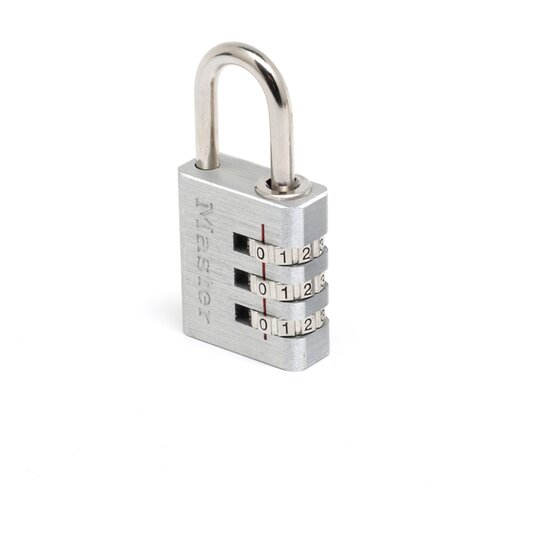
\includegraphics[scale=0.65]{hengelas}
\end{figure}

\eksop{1PV17D1}{1PV17D1opg8}
Ved en skole leser 80 \% av elevene aviser på nett, 50\% les erpapiraviser, og 2\% leser ikke
aviser. \os

a) Systematiser opplysningene gitt i teksten over i et venndiagram eller i en
krysstabell. \os

b) Bestem sannsynligheten for at en tilfeldig valgt elev ved skolen leser både aviser på nett og papiraviser.\os

En elev ved skolen leser aviser på nett.\os

c) Bestem sannsynligheten for at denne eleven ikke leser papiraviser.


\grubeksoprecc{gv25d2opg4}{GV25D2}
Vurder om påstandene er riktige eller ikke. Grunngi svaret ditt.\os

''Ved et terningkast er det lik sjanse for å få et partall eller et oddetall.'' \os
''I en skål er det to gule baller og to røde baller. Ved å trekke opp to baller, er det sjansen for at ballene har lik farge like stor som sjansen for at de har ulik farge.''
\end{document}


